\section{Charged Particle Tracking System}
\label{sec:tracker}
The charged particle tracking system is the sub-detector that lies closest to the beam pipe.
Its purpose is to measure the the trajectories of charged particles that emerge from the collisions.
The trajectories are then used to determine the momentum and charge of the charged particles.
In order to measure the trajectories several layers of silicon detectors are used, as charged particles traverse these layers they create electronic signals in the silicon.
Each of these signals, often referred to as ``hits'', correspond to the position of a charged particle as it travels through the detector.
The hits that are measured in the tracking system are fit to a helix producing the trajectories that are used to measure the charge and momentum.
For high momentum tracks the tracking system provides very good resolution for the transverse momentum of approximately $1-2\%$ in the barrel region, while in the endcap region ($|\eta| > \sim1.5$) the resolution degrades as can be seen in Figure \ref{fig:trackerptres}.
\begin{figure}[htpb]
\begin{center}
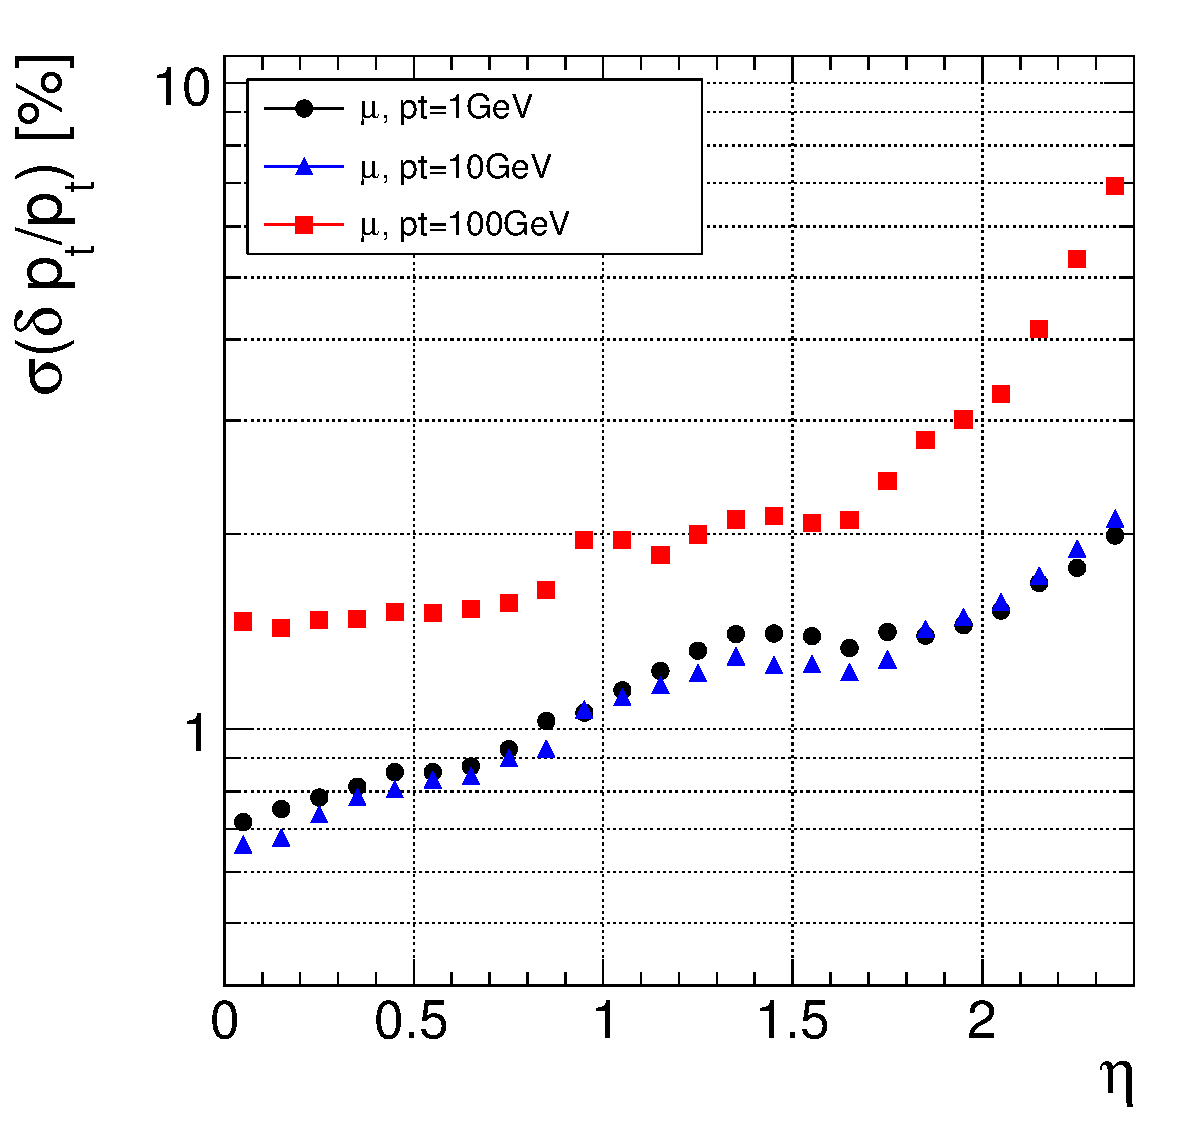
\includegraphics[width=0.85\textwidth]{plots/trackerptres.pdf}
\caption{Transverse momentum resolution of the CMS tracking system as a function of pseudo-rapidity ($\eta$) for muons with $p_{T} = 1$, $10$, and $100$ GeV\cite{CMS_DETECTOR}.}
\label{fig:trackerptres}
\end{center}
\end{figure}

The tracking system is designed to have the capacity of measuring secondary decay vertices, for example, arising from the decay of bottom quarks and tau leptons.
Bottom quarks and tau leptons have relatively long life times, as such they travel a non-negligible distance before decaying, giving rise to secondary decay vertices.
In order to measure secondary decay vertices, the tracking system is constructed using two technologies, an inner tracking system consisting of silicon pixel detectors and an outer tracking system of silicon strips.
The inner layer of the pixel tracking system is placed at a radius of $4.4$ cm in order to be as close as possible to the interaction point.
This pixel tracking system is made up of three layers in the barrel and two layers in the endcaps.
Outside the pixel tracking system is the silicon strip tracking system consisting of ten layers of silicon strips in the barrel region and 12 layers in the endcaps. 
A schematic of the CMS tracking system can be seen in Figure \ref{fig:trackerlayout}.
The transverse impact parameter ($d_{0}$) resolution of the tracking system gives an indication of the performance one can expect for the secondary decay vertex reconstruction, for high momentum tracks the resolution is approximately $10$ \micrometer as can be seen in Figure \ref{fig:trackerd0res}. %FIXME micrometer
For lower momentum tracks the resolution of $d_{0}$ degrades due to multiple scattering of the particle in the tracker material.
\begin{figure}[htpb]
\begin{center}
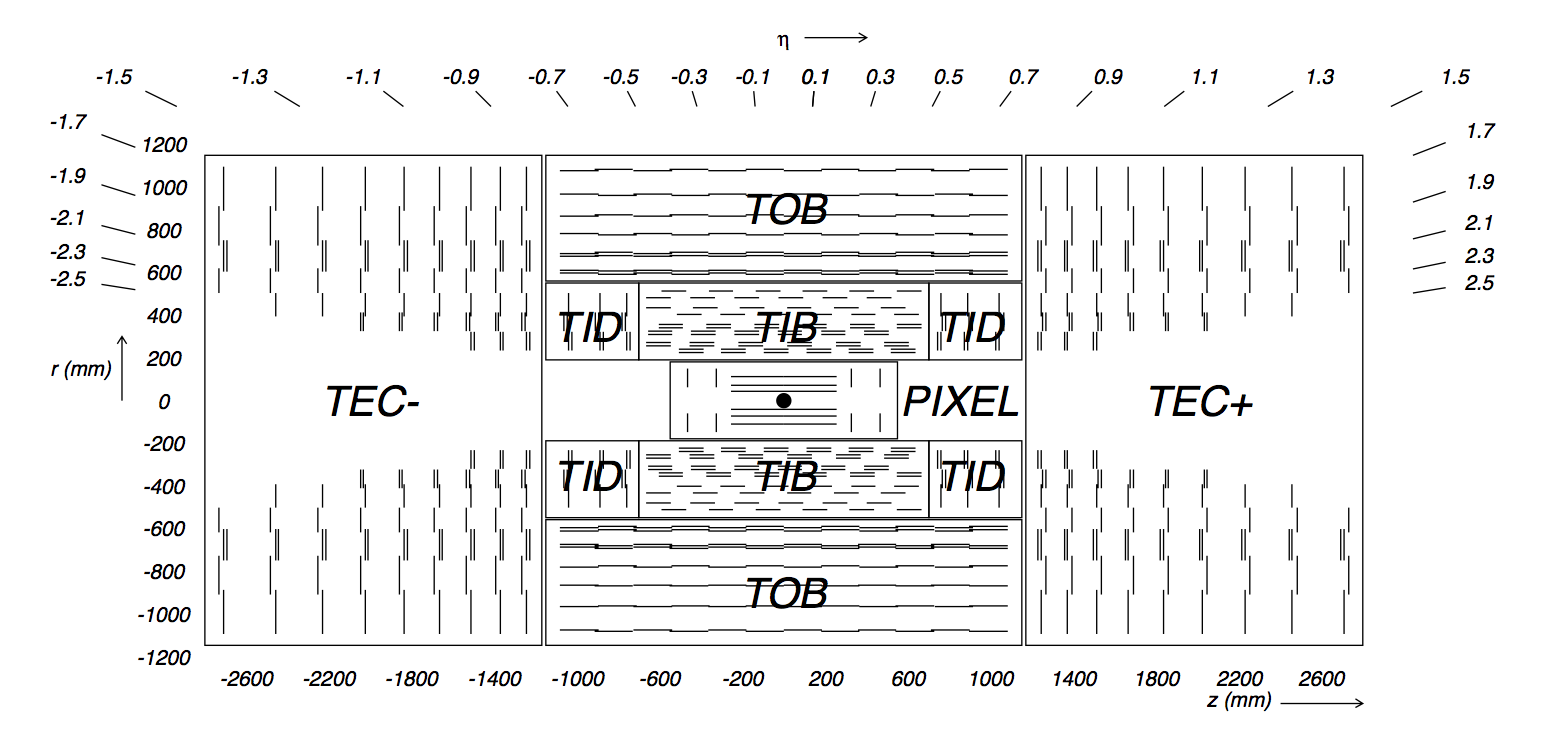
\includegraphics[width=0.85\textwidth]{plots/trackerlayout.png}
\caption{Schematic of the CMS inner tracking system\cite{CMS_DETECTOR}. The barrel tracker is divided into the Tracker Inner Barrel (TIB) and Tracker Outer Barrel (TOB). The endcap tracker is divided into the Tracker End Cap (TEC) and Tracker Inner Disks (TID).}
\label{fig:trackerlayout}
\end{center}
\end{figure}

\begin{figure}[htpb]
\begin{center}
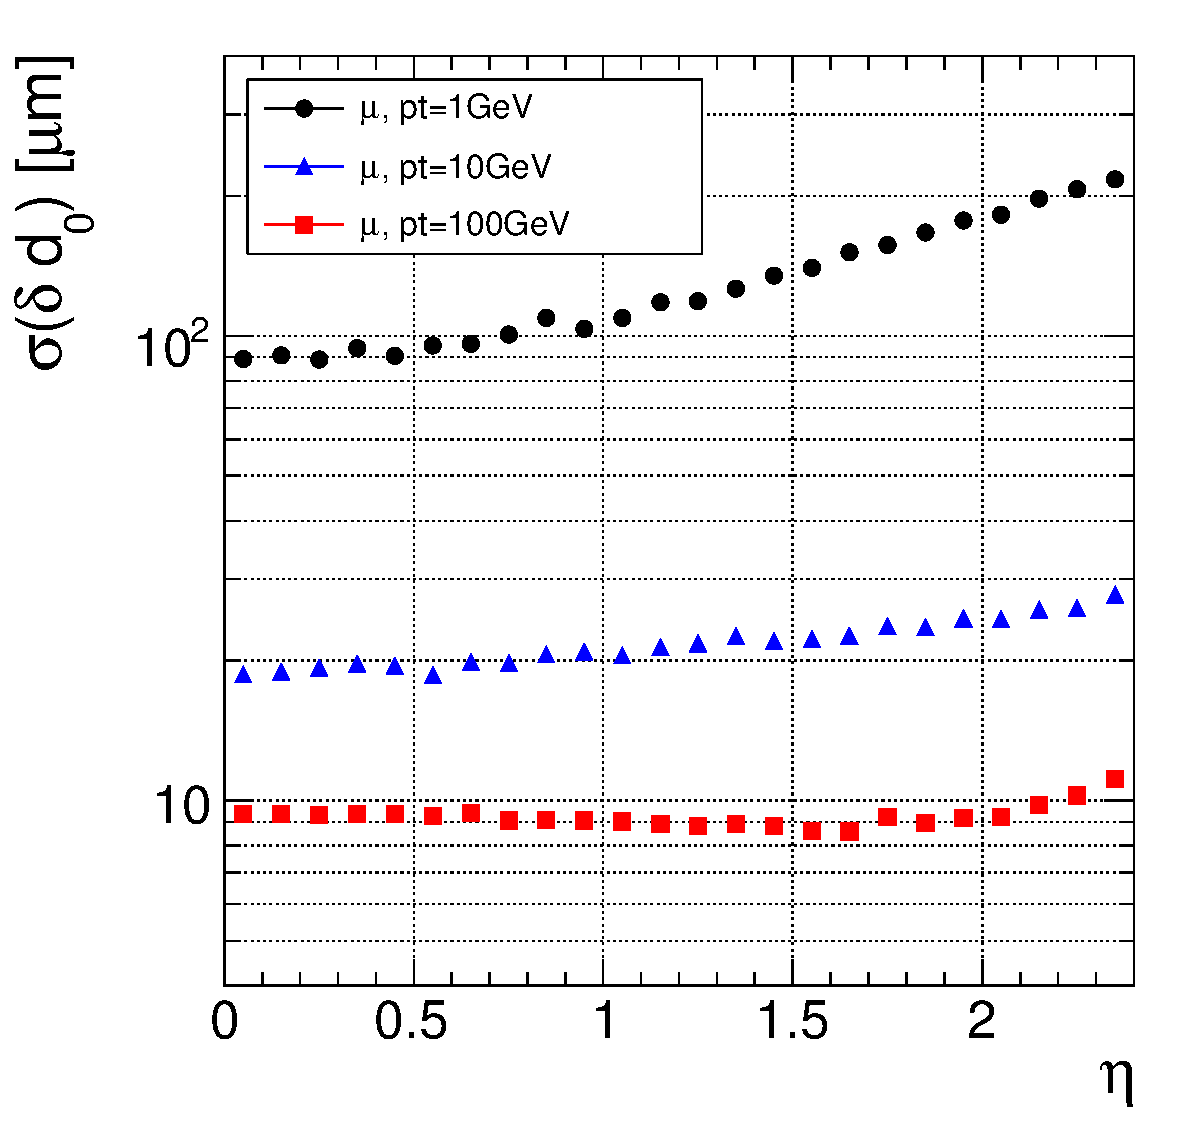
\includegraphics[width=0.85\textwidth]{plots/trackerd0res.pdf}
\caption{Transverse impact parameter resolution of the CMS tracking system a function of pseudo-rapidity ($\eta$) for muons with $p_{T} = 1$, $10$, and $100$ GeV\cite{CMS_DETECTOR}.}
\label{fig:trackerd0res}
\end{center}
\end{figure}

Both the inner and outer tracking systems consist entirely of silicon, which operate by doping the silicon and thus creating a diode. % FIXME reword?
A reverse bias is then applied to the silicon to deplete the region, so that when a charged particle passes through the silicon a small ionization current is induced which can then be measured.
The most common method of forming this type of silicon diode is to create a p-n junction, however to ensure radiation hardness the layering in the tracking system silicon is more complicated\cite{CMS_DETECTOR}. %FIXME involves creating
In order to achieve high resolution track measurements suitable for the measurement of secondary decay vertices and particle impact parameters, the pixels in the inner layers are electronically isolated and constructed in sizes of $100$x$150$ \micrometer.
The tracking system was designed such that the occupancy would be less than or equal to 1\% at the design luminosity, and as such the outer tracking system does not need to be as finely divided as the inner pixel system.
The outer tracking system is constructed of silicon strips providing single point resolution between $23$ to $52$ \micrometer in both $r$-$\phi$ and $z$ directions.

Tracks are reconstructed from the reconstructed hits in the tracker by means of the Combinatorial Track Finder (CTF) algorithm\cite{TRACKRECO}.
The CTF begins by first locating pairs of reconstructed hits in the inner pixel detector that are compatible with the interaction region.
The track finding then uses a Kalman filtering method to combine the seeded parameters with nearby reconstructed hits.
During each step of the finding algorithm each track is assigned a quality, ambiguities that arise from two tracks are resolved by rejecting the track that is of lesser quality.
Once the track finding method is complete each track undergoes two least squares fitting procedures, the first is an inside-out fit that serves to remove any approximations or biases that arise from the seeding or finding algorithms.
The second fit is an outside-in fit that serves to smooth the final track.
The final track finding procedure is performed iteratively to improve the efficiency of the track finding process, the CTF is repeated three to four times.
After each iteration of the CTF a set of filters is applied setting aside high quality tracks and removing their reconstructed hits from the next iteration.
The iterative procedure has been shown to increase the track finding efficiency by approximately $5\%$ while keeping mis-identification rates low.
Further, the iterative procedure also allows for the reconstruction of low momentum tracks that would otherwise not be reconstructed with a single CTF.
